\lfoot{Autor: Who?}
\subsubsection{Kompatible Geräte}
\label{subsec:device-compability}

Android kann auf vielen verschiedenen Plattformen, von Handys zu Tabletts laufen.
Als Entwickler bietet die Palette von Geräten ein enormes potenzielles Publikum.
Um auf all diesen Oberflächen reibungslos zu funktionieren sollte es einige Feature Variabilitäten tolerieren und eine 
flexlible Benutzeroberflaeche zur Verfuegung stellen. 

Um das zu ermöglichen bietet Android die möglichkeit, verschiedene XML Layouts zu erstellen um verschiedene Bildschirmgrößen anzusprechen.

Beim Programmieren der App, kann auch die Minimum und Maximum Version des Devices eingestellt werden, wobei wir hier eine größere Menge an Nutzern erzielen wollen. 

\begin{figure}[!htb]\centering
	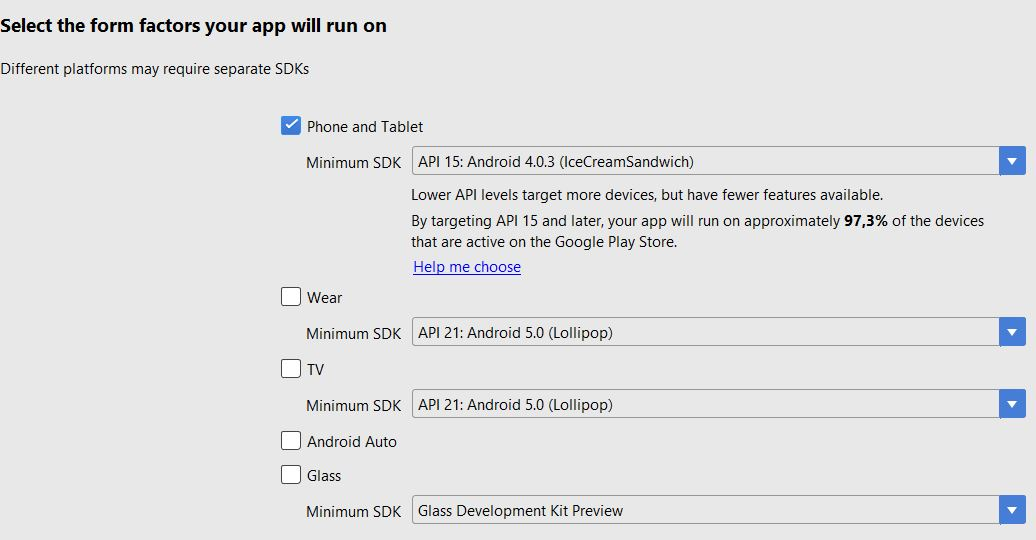
\includegraphics[width=1.0 \textwidth]{images/MinMaxVers}
	\caption{Version}\label{Fig:Version}
\end{figure}



\clearpage % DO NOT REMOVE